\documentclass[10pt,a4paper]{article}


%%%PACKAGES
\usepackage[utf8]{inputenc}
\usepackage[T1]{fontenc}
\usepackage[french]{babel}
\usepackage{multicol}
\usepackage[left=2.1cm, right=2.1cm, bottom=2.7cm, top=2.7cm]{geometry}
\usepackage{titling}
\usepackage{xcolor}
\usepackage{fancyhdr}
\pagestyle{fancy}
\usepackage{fancybox}
\usepackage{lastpage}
\usepackage{stmaryrd}
\usepackage[normalem]{ulem}
\usepackage{graphicx}
\usepackage{soul}
\usepackage{float}
\usepackage{amsmath,amsfonts,amsthm,amssymb} 
\usepackage{mdframed}
\usepackage{enumitem}
\usepackage{changepage}
\usepackage{titlesec}
\usepackage[most]{tcolorbox}
\usepackage{tabto,lipsum}
\usepackage{marginnote}[] %%%pour les symboles dans la marge
\usepackage{tasks} % pour aligner des enumerate
\usepackage{framed}

%%%PACKAGE SYMBOLES
\usepackage{pifont}
\usepackage{fourier}
\usepackage{ticollege} %pour le symbole calculatrice

%%%PACKAGES TIKZ
\usepackage{tikz}
\usepackage{pstricks}
\usepackage{pstricks-add}
\usetikzlibrary{arrows}
\usepackage{mathrsfs}
\usepackage{pgfplots}
\pgfplotsset{compat=1.15}




%%%RACCOURCIS
\newcommand{\N}{\mathbb{N}}
\newcommand{\Z}{\mathbb{Z}}
\newcommand{\Q}{\mathbb{Q}}
\newcommand{\R}{\mathbb{R}}
\newcommand{\C}{\mathbb{C}}
\newcommand{\oa}{\overrightarrow}
\newcommand{\ol}{\overline}


%%% en haut et en bas
\fancyhf{}
\fancyhead[L]{\type}
\fancyhead[R]{\niveau}
\fancyfoot[L]{Ch.\numchap : \titrechap}
\fancyfoot[R]{\thepage \hspace{1pt} / \pageref{LastPage}}


%%%ENCADRÉS
%énoncés importants
\newcommand{\cbox}[1]{\begin{tcolorbox}[lower separated=false, colback=white]
#1
\end{tcolorbox}}
%%%LEFTBAR
\renewenvironment{leftbar}{%
  \def\FrameCommand{\hspace{1cm}\vrule width 0.4pt \hspace{10pt}}%
  \MakeFramed{\advance\hsize -\width\FrameRestore}}%
 {\endMakeFramed}



\setlength\parindent{0pt}


%%% STYLE DES SECTIONS
\renewcommand\thesection{\Roman{section}.}
\renewcommand\thesubsection{\arabic{subsection}.}
\renewcommand\thesubsubsection{\alph{subsubsection})}

\titleformat{\section}
  {\scshape \Large \bfseries}{\thesection}{1em}{}
\titleformat{\subsection}
  {\normalfont  \large \bfseries}{\thesubsection}{1em}{}
\titleformat{\subsubsection}
  {\normalfont\large }{\thesubsubsection}{1em}{}

%%%STYLE DES ITEMIZE
\setitemize[1]{label=\textbullet}


%%%THEOREM STYLES

\newtheoremstyle{exercices}
{}                % Space above
{}                % Space below
{}        % Theorem body font % (default is "\upshape")
{}                % Indent amount
{\bfseries}       % Theorem head font % (default is \mdseries)
{}               % Punctuation after theorem head % default: no punctuation
{10pt}               % Space after theorem head
{}                % Theorem head spec
\theoremstyle{exercices}
\newtheorem{exo}{Exercice}

\newtheoremstyle{enonce}
{}                % Space above
{}                % Space below
{}        % Theorem body font % (default is "\upshape")
{}                % Indent amount
{\bfseries}       % Theorem head font % (default is \mdseries)
{ :}               % Punctuation after theorem head % default: no punctuation
{3pt}               % Space after theorem head
{}                % Theorem head spec
\theoremstyle{enonce}
\newtheorem*{defi}{Définition}
\newtheorem*{defis}{Définitions}
\newtheorem*{prop}{Propriété}
\newtheorem*{props}{Propriétés}
\newtheorem*{thm}{Théorème}
\newtheorem*{defiprop}{Définition-propriété}

\theoremstyle{remark}
\newtheorem*{demo}{Démonstration}
\newtheorem*{exple}{Exemple}
\newtheorem*{exples}{Exemples}
\newtheorem*{rem}{Remarque}
\newtheorem*{rems}{Remarques}
\newtheorem*{note}{Notation}
\newtheorem*{met}{Méthode}
\newtheorem*{app}{Application}
\newtheorem*{ill}{Illustration géométrique}

%%%TITRE
\newcommand{\montitre}[1]{
\begin{center}
%\vspace{-0.5cm}
\doublebox{
 \Large \scshape 
 #1}
\end{center}
}


%%%CITATION
\renewcommand{\citation}[4]{
\begin{minipage}{0.25\textwidth}
\hspace{1pt}
\end{minipage} \hfill
\begin{minipage}{0.7\textwidth}
\center
\small
\og #1 \fg{}
\flushright {\footnotesize \textsc{#2}, \textit{#3} (#4)}
\end{minipage}\\[\baselineskip]
}


%%%SYMBOLES MARGE
\newcommand{\acomp}{\reversemarginpar
\marginnote{\leafNW}}

\newcommand{\attention}{\reversemarginpar
\marginnote{\warning}}

\newcommand{\PCQCI}{\reversemarginpar
\marginnote{\ding{106}}}

\newcommand{\todo}{\reversemarginpar
\marginnote{\ding{217}}}

\newcommand{\calc}{\reversemarginpar
\marginnote{\TiCCalc*[calcscale=0.4, calcrotate=0]}}




%%%à modifier à chaque fois
\newcommand{\type}{Exercices}
\newcommand{\niveau}{Seconde}
\newcommand{\numchap}{1}
\newcommand{\titrelongchap}{Proportions}
\newcommand{\titrechap}{Proportions}
%\newcommand{\titre}{Feuille mixte cours et exo} %par exemple : \newcommand{\titre}{Chapitre \numchap : \titrechap}
%%%%%%%%%%%%%%%%
\begin{document}



\montitre{Fiche d'exercices : \titrechap}
\cbox{
\textit{Capacités attendues :}

\begin{itemize}
    \item Exploiter la relation entre effectifs, proportions et pourcentages
    \item Traiter des situations simples mettant en jeu des pourcentages de pourcentages
\end{itemize}
}

\subsection{Sans calculatrice}
 \begin{exo}
A la rentrée 2023, en ligue 1 de football, il y a 9 entraineurs français sur un total de 18 entraineurs de club. Quelle proportion d'entraineurs français y a-t-l en ligue 1 de football ?
\end{exo}  

\begin{exo}
 Un commerçant souhaite vendre un chocolat chaud à 3€ hors taxes.  La taxe sur la valeur ajoutée (TVA) pour les boissons non alcoolisées est de $10\%$. Combien vaut le chocolat chaud avec la TVA ? Peut-on dire que lorsque je paie mon chocolat chaud, je paie 10\% de TVA ?
\end{exo}
 
   \begin{comment}
\begin{exo}
     
Un club d'athlétisme compte 150 adhérents, parmi eux 25 pratiquent le saut à la perche. Quelle est la proportion d'adhérents qui pratiquent le saut à la perche?

\end{exo}
   \end{comment}




\begin{exo}
\textbf{QCM}

\medskip

Pour chacune des questions de ce questionnaire à choix multiples, une seule réponse est exacte.
\medskip
\begin{enumerate}
\begin{comment}
     \item Parmi les 812 adhérents d'un association 200 sont des hommes. Quel est le pourcentage d'hommes dans cette association?
    \begin{tasks}(5)
        \task $10,3\%$
        \task $24,6\%$
        \task $54,1\%$
    \end{tasks}

\end{comment}
   
    \item Parmi les 1057 élèves du lycée GT, 333 sont en seconde. Quel est le pourcentage d'élèves en seconde ?
    \begin{tasks}(5)
        \task $10,3\%$
        \task $31,5\%$
        \task $49,1\%$
    \end{tasks}

    \item En 2015 la ville de Saint-Denis comptait 111 103 habitants, parmi lesquels $51,86\%$ environ vivaient dans les quartiers "La plaine", "Grand centre ville" et "Franc-Moisin - Bel Air - Stade de France" . Quel est le nombre d'habitants qui vivaient dans ces quartiers en 2015 ? (Source : \textit{INSEE})
    \begin{tasks}(5)
        \task 26 343
        \task 52 503
        \task 57 615
    \end{tasks}

\end{enumerate}
\end{exo}


\subsection{Avec calculatrice}

\begin{minipage}{0.5\textwidth}
    
    \begin{exo}
    A l'aide de la figure \ref{ac} ci-contre, répondre aux questions suivantes :
    \begin{enumerate}
        \item Quelle est la proportion de lycées polyvalents parmi les lycées de l'académie ?
        \item Quelle est la part des personnels qui n'est pas enseignant ?
        \item Dans l'académie de Créteil, y a-t-il plus de lycées professionnels dans le public ou le privé ?
    \end{enumerate}
\end{exo}

 \begin{exo}
        Pour une personne seule, gagnant moins de 27 478€ par an, l'impôt sur le revenu fonctionne de la manière suivante :
        \begin{itemize}
            \item Les premiers 10 777€ sont imposés à $0$\%
            \item De 10 778€ à 27 478€, le taux d'imposition est de $11$\%
        \end{itemize}

        Combien paiera d'impôts une personne ayant gagné 8 000€ dans l'année ? Et une personne ayant gagné 25 000 € ? 
    \end{exo}
\end{minipage}
\hfill
\begin{minipage}{0.45\textwidth}
\begin{figure}[H]
    \centering
    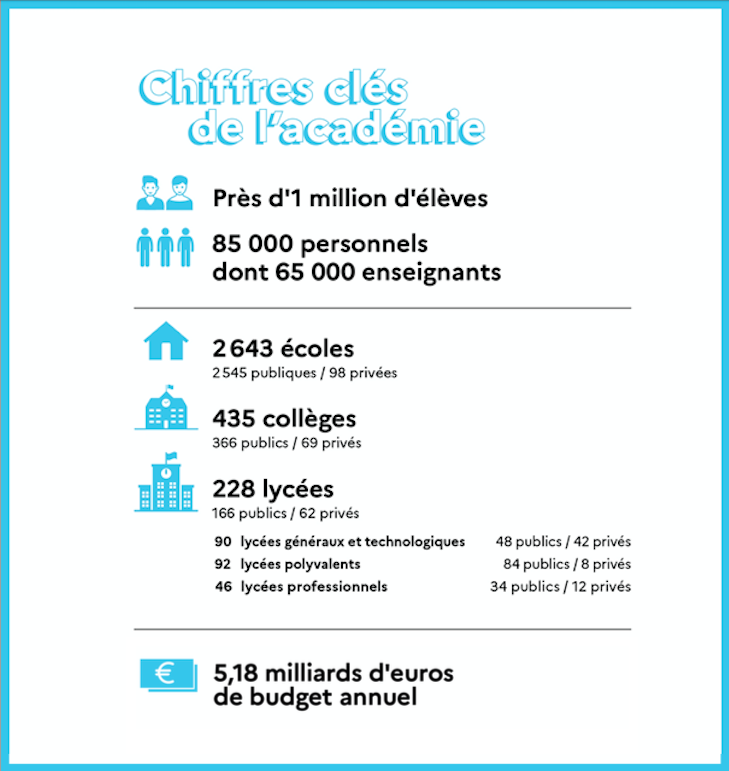
\includegraphics[width=\textwidth]{chiffres-aca.png}
    \caption{Source : rectorat de Créteil}
    \label{ac}
\end{figure}
\end{minipage}

\begin{exo}
En France métropolitaine, sur le troisième trimestre 2018, le taux de chômage correspond à $8$ \% de la population active. On compte $2,6$ millions de chômeurs. À combien s’élève la population active à cette date ?
\end{exo}

\begin{exo}
    D'après l'étude The Global Human Day du PNAS, les humains passent en moyenne 9h 6min par jour à dormir. Quelle proportion du temps passent-ils éveillés, en moyenne ?
\end{exo}

\begin{exo}
    L'algorithme ci-dessous permet de retrouver le résultat de l'exercice 2. Réécrire l'agorithme pour qu'il calcule le prix TTC d'un café à $1,50$€.
   
$a \leftarrow 0,1$
$b \leftarrow  3$
$c \leftarrow a \times b$
$d \leftarrow b + c$

\end{exo}

\begin{exo}
    Trois amis A, B et C décident de faire un repas commun.
A apporte 5 plats ; B en apporte 3. C n'apporte rien, mais dit qu'il remboursera ses amis. En supposant que tous les plats ont la même valeur, C verse en accord avec les autres 16 €. Comment répartir cette somme équitablement ?
\end{exo}

\begin{exo}
Au lycée, $31,5$\% des élèves sont en filière technologique, parmi lesquels $25,5$\% sont en section STI2D. Quelle est la proportion d'élèves en STI2D au lycée ?
\end{exo}

\begin{exo}
D'aprés les statistiques de l'Insee, la France comptera 74 millions d'habitants en 2050. Parmi les Français, les personnes de plus de 65 ans représenteront 40 \%. De plus, 60 \% des plus de 65 ans auront plus de 75 ans. Quelle sera la proportion de Français âgée de plus de 75 ans en 2050 ? Donner le résultat en pourcentage.
\end{exo}

\begin{minipage}{0.6\textwidth}
    \begin{exo}
    Les affirmations suivantes sont-elles vraies ou fausses ? Justifier, sans calculatrice :
    \begin{enumerate}
        \item \textit{Affirmation :} Pour calculer la superficie des territoires indigènes (voir figure \ref{Amazonie} ci-contre) en région amazonienne, on effectue le calcule $\displaystyle 8470209 \times \frac{28,6}{100}$.
        \item La part des filles choisissant l'enseignement de spécialité mathématiques en première générale est de $61,4\%$ (source : MENJ-DEPP). 
        
        \textit{Affirmation :} On peut en déduire que la part de garçons choisissant l'enseignement de spécialité mathématiques est de $38,7\%$.
        \item Dans la recette du quatre-quart, il faut mettre un quart de beurre, un quart de sucre, un quart de farine et un quart d'oeufs. 
        
        \textit{Affirmation :} Si je rajoute à la recette d'origine 60g de beurre, de sucre, de farine, et d'oeuf, le gateau est toujours un quatre-quart.
        \item \textit{Affirmation :} 70\% de 40\% c'est la même chose que 40\% de 70\%.
    \end{enumerate}
\end{exo}
\end{minipage}
\hfill
\begin{minipage}{0.37\textwidth}
\begin{figure}[H]
    \centering
    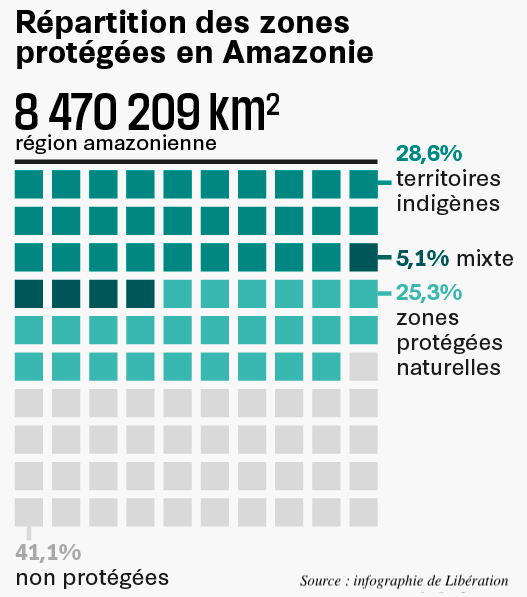
\includegraphics[width=.95\textwidth]{foret-amazonienne.png}
    \caption{Extrait d'une infographie du journal \textit{Libération} : "La perte du couvert forestier en Amazonie"}
    \label{Amazonie}
\end{figure}
\end{minipage}

\end{document}
